\documentclass[12pt]{article}

\usepackage[utf8x]{inputenc} % Включаем поддержку UTF8  
\usepackage[russian]{babel}  % Включаем пакет для поддержки русского языка  
\usepackage{hyperref}        % Для гиперссылок

% Математика
\usepackage{amsmath,amsfonts,amssymb,amsthm,mathtools} % AMS
\usepackage{icomma}
\usepackage{mathrsfs}

\usepackage{xcolor}

% Прога
\usepackage{etoolbox}
\usepackage{listings}

\definecolor{codegreen}{rgb}{0,0.6,0}
\definecolor{codegray}{rgb}{0.5,0.5,0.5}
\definecolor{codepurple}{rgb}{0.58,0,0.82}
\definecolor{backcolour}{rgb}{0.95,0.95,0.92}

\lstdefinestyle{mystyle}{
	backgroundcolor=\color{backcolour},   
	commentstyle=\color{codegreen},
	keywordstyle=\color{magenta},
	numberstyle=\tiny\color{codegray},
	stringstyle=\color{codepurple},
	basicstyle=\ttfamily\footnotesize,
	breakatwhitespace=false,         
	breaklines=true,                 
	captionpos=b,                    
	keepspaces=true,                 
	numbers=left,                    
	numbersep=5pt,                  
	showspaces=false,                
	showstringspaces=false,
	showtabs=false,                  
	tabsize=2
}

\lstset{style=mystyle}

% Цвета
\usepackage{xcolor}

% Картинки
\usepackage{graphicx}
\graphicspath{ {./images/} }

\usepackage{tikzsymbols}

% Работа с таблицами
\usepackage{array,tabularx,tabulary,booktabs} % Дополнительная работа с таблицами
\usepackage{longtable}  % Длинные таблицы
\usepackage{multirow} % Слияние строк в таблице

% Нумерованные списки
\usepackage[shortlabels]{enumitem} % Разные лейблы

% Текст
\usepackage[normalem]{ulem}  % для зачеркивания текста

\newtheorem{property}{Свойство}
\newtheorem{consequence}{Следствие}[property]

\begin{document}
	
	\thispagestyle{empty}
	\begin{center}
		\textbf{ПРАВИТЕЛЬСТВО РОССИЙСКОЙ ФЕДЕРАЦИИ}
		
		\vspace{5ex}
		
		\textbf{Федеральное государственное автономное образовательное учреждение \\ высшего образования \\ <<Национальный исследовательский университет \\ <<Высшая школа экономики>>}
	\end{center}
	\vspace{5ex}
	
	\begin{center}
		Московский институт электроники и математики им. А.Н. Тихонова  
		
		\vspace{5ex}
		
		Департамент прикладной математики
		
		\vspace{10ex}
		\textbf{Отчёт \\ по лабораторной работе A2 \\ по курсу <<Компьютерный практикум>> \\ Задание № 13}
		\vspace{7ex}
		
	\end{center}
	
	\begin{center} 
		\begin{tabular}{| p{0.3\linewidth}| p{0.3\linewidth}| p{0.3\linewidth}|}
			\hline	
			ФИО студента & Номер группы & Дата \\  \hline
			& & \\  
			Кейер Александр \newline Петрович & БПМ-231 & \today \\  
			& & \\  \hline		
		\end{tabular}
	\end{center}
	
	\begin{center}
		\vspace{3ex}
		
		\vfill
		
		\normalsize
		
		\textbf{Москва, 2023}
	\end{center}
	
	\newpage
	
	%---------------------------------------------------------------------------------
	
	\section*{Задание}
	
	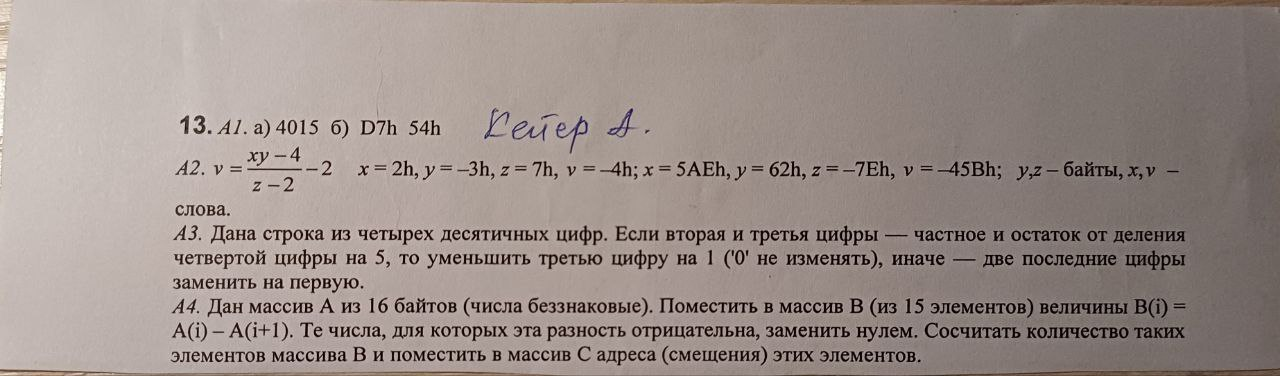
\includegraphics[width=400pt]{variant_13.jpg}
	
	$$v = \frac{xy - 4}{z - 2} - 2$$
	$$x = 2h, y = -3h, z = 7h, v = -4h$$
	$$x = 5AEh, y = 62h, z = -7Eh, v = -45Bh$$
	\begin{center}
		$y, z$ - байты; $x, v$ - слова
	\end{center}
	
	\newpage
	
	%---------------------------------------------------------------------------------
	
	\section*{Решение}\addcontentsline{toc}{section}{}
	
	\begin{lstlisting}[language=C]
	#include <stdio.h>
	
	int testCounter = 1;
	
	void test(short int x, char y, char z, short v) {
		printf("\n");
		
		short v_c, v_as;
		
		__asm__(
			"# calculating numerator \n\n"
			
			"\t mov al, %2       # y --> al \n"
			"\t cbw              # y --> word \n"
			"\t imul %1          # x * y \n"
			"\t sub ax, 4        # ax - 4 --> ax \n"
			"\t mov bx, ax"
			
			"\t # calculating denominator \n\n"
			
			"\t mov al, %3       # z --> dl \n"
			"\t cbw              # z --> word \n"
			"\t sub ax, 2        # dx - 2 --> dx \n\n"
			"\t xchg ax, bx      # ax <--> bx \n"
			
			"\t idiv bx          # ax / bx --> ax \n"
			"\t sub ax, 2        # ax - 2 --> ax \n\n"
			
			"\t mov %0, ax       # ax --> v"
			
			: "=m" (v_as)                
			: "m" (x), "m" (y), "m" (z)  
		);
		
		v_c = ((short)y * x - 4) / ((short) z - 2.0) - 2;
		
		printf("Test %d\n", testCounter++);
		printf("Assembler result: %d (10-system) or %hx (16-system)\n", v_as, v_as);
		printf("C result: %d or %hx\n", v_c, v_c);
		printf("Correct values: %d or %hx\n", v, v);
		
		printf("\n");
	}
	
	int main() {
		test(0x2, -0x3, 0x7, -0x4);
		printf("===========\n");
		test(0x5AE, 0x62, -0x7E, -0x45B);
		
		return 0;
	}
	\end{lstlisting}
	
	\newpage
	
	%---------------------------------------------------------------------------------
	
	\section*{Тесты}\addcontentsline{toc}{section}{}
	
	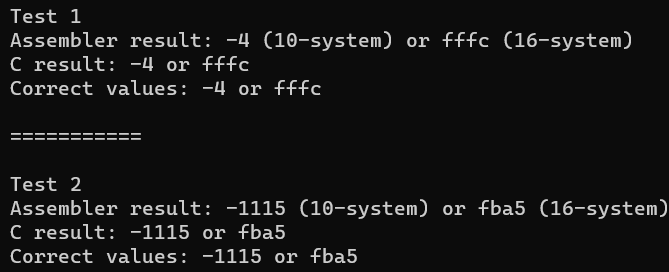
\includegraphics[width=400pt]{tests.png}
	
	\noindent Так как ответ получен в виде дополнительного кода, то преобразуем его руками, чтобы проверить правильность ответа: \newline
	$fffc_{16} \to 1111\ 1111\ 1111\ 1100_2 \to -(100_2) \to -4_{16}$ -- верно \newline
	$fba5_{16} \to 1111\ 1011\ 1010\ 0101_2 \to -(-10001011011_2) \to -45b_{16}$ -- верно
	
\end{document}
